\section{Problem Definition} \label{sec:prob}
In this section, we focus on describing the identified performance issues: 1) long execution paths of the guest page table (de)allocation and 2) the additional IOTLB flushes.
As Xen~\cite{XEN-SOSP03} is a typical and popular paravirtual hypervisor, in this section we use Xen in a x86 MMU model~\cite{x86-pv-model} to illustrate the details. 
It is easy to map the descriptions into the corresponding mechanisms on other paravirtual hypervisors.

\subsection{Long Execution Path}\label{sec:longpath}

\subsubsection{Costly Memory Allocators}
To allocate or free a page-table page, the guest kernel has to invoke the system allocators, typically from slab allocator to buddy allocator.
Each of these allocators maintains a set of complex data structures to track the internal status.
%not only returns or release the page, the internal status will be updated correspondingly.
any allocation and deallocation invocation will trigger the updates of such data structures. 
% in addition, to support multicore setting, such allocators have to leverage locks to prevent race conditions.
% in one invocation, there will be many locks locked and unlocked 

All these increase the invocation time.
In fact, it is not 

\subsubsection{Security Validations}

\paragraph{Page Table Validations}\label{sec:pv-security}

Page tables are used by a hardware, i.e., Memory Management Unit (MMU), to translate the linear addresses into physical addresses used by the hardware to execute instructions.
In the PAE-enabled paging mode, a page table has three levels: L1 level (bottom level), L2 level (middle level) and L3 level (top level).
The slots in L1, L2 and L3 levels are known as Page Table Entry (PTE), Page Middle Directory (PMD) and Page Global Directory (PGD), respectively.
A PTE slot could determine the access permissions of a page, e.g., the kernel could set a page as read-only by clearing the bit within a PTE slot that represents the writable permission.

There are many page tables in a guest VM, as each user process has its own page tables.
The creation and exit of a user process will be accompanied by the creation and destruction of a page table respectively.
It means that if there are numerous temporary processes generated within a period, there will be a large number of page tables created.

In order to ensure that the guest cannot subvert the system, Xen requires that certain update policies are maintained,
and thus all updates of the page tables should be vetted by Xen.
To this end, the guest OS is deprivileged, from ring-0 to ring-1, leaving ring-0 for the Xen hypervisor.
This prevents the guest OS from executing privileged instructions, e.g., the guest OS cannot directly update control registers.

Xen also defines a number of page types, which are listed in Table~\ref{tab:pagetype}, and maintain a type reference count for each page.
Xen enforces the policies that any given page has exactly one type at any given time,
and only pages with the writable type have a writable mapping in the page tables.
By doing this it can ensure that the guest OS is not able to directly modify any page-table pages and therefore subvert the security of the whole system.
If the guest kernel attempts to update the page table, it has to issue a hypercall to ask the hypervisor to complete the update.
As Xen is always involved in all updates of the page tables, the policies on the page table updates are non-bypassable.

Whenever a page table is loaded into the hardware page-table base register (cr3),
the hypervisor takes an appropriate type reference with the L3 page-table type.
If the page is not already of the required type, then in order to take the initial reference it must first have a type count of zero.
In addition, it must be validated to ensure that it follows the following policy:
for a page with a page-table type to be valid, it is required that any pages referenced
by a present page table entry in the page have the type of the next level down.
For instance, any page referenced by a page with type L3 Page Table must itself have the type L2 Page Table.
This policy is applied recursively down to the L1 page table layer.
At L1 the invariant is that any data page mapped by a writable page table entry must have the writable page type.
By applying these policies, Xen ensures that all page-table pages as a whole are safe to be loaded into the cr3.
Similar requirements are also placed on other special page types, e.g., GTD/LDT pages.

The page type is allowed to be changed.
Xen enforces that the type of a page can only be changed when the type count is zero.
In addition, Xen also requires that every page type update only occur between writable and non-writable pages, as summarized in Figure~\ref{fig:page-type-updates}.

\begin{figure}[ht]
\centering
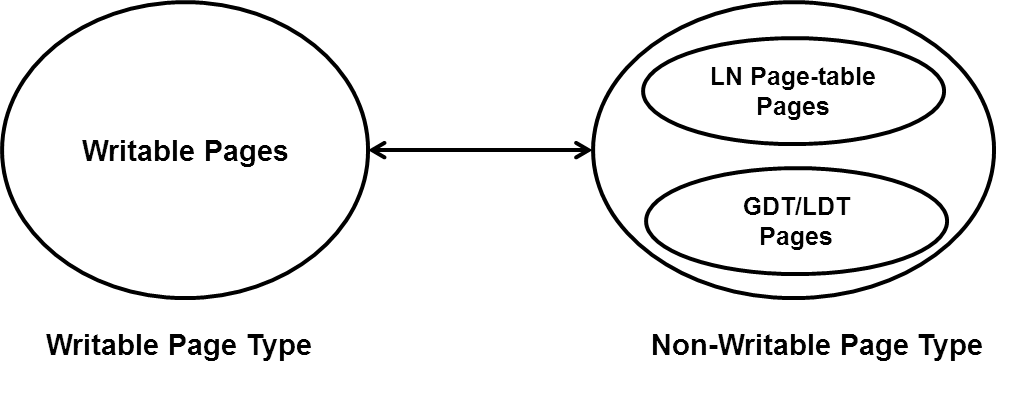
\includegraphics[width=0.45\textwidth]{image/background/page-type-updates.png} \\
\caption{Page Type Updates between writable pages and non-writable pages. (Writable pages are writable for both software and DMA
while non-writable pages are inaccessible to them.)}
\label{fig:page-type-updates}
\end{figure}


\paragraph{DMA Validations}

\subsection{Additional IOTLB Flush Issue}
The dependency between the guest page table and the IOTLB is very subtle.
To fully understand the dependency, we need to know the details about how the paravirtualized hypervisor protects itself through guest page table and IOMMU.
Specifically, we explicitly describe 1) paravirtualized MMU mode, and 2) IOMMU and DMA address translation.

\subsubsection{DMA Address Translation}
%citing: intel vt-d
The input/output memory management unit (IOMMU)~\cite{directio} is a memory management unit (MMU) that connects a DMA-capable I/O bus to the main memory.
Like a traditional MMU, the IOMMU maps device addresses (also called as I/O addresses) to physical addresses through a dedicated page table.
This technique is also known as DMA remapping.
The IOMMU page table that is created and maintained by the hypervisor in its own space, is able to restrict the access on a particular page by configuring the permission bits.
The hypervisor grants different access permissions for different page types, such as the writable pages are always allowed full access permissions, while the page-table pages are always inaccessible to any devices.
This is why when the page-type changes between writable page and page-table page, updating IOMMU page table is always necessary.

However, the DMA remapping always needs the page table walking, which is slow and inefficient.
To accelerate the translation speed, the I/O translation look-aside buffer (IOTLB) is introduced.
The IOTLB is used to cache frequently accessed page table entries.
By doing so, the IOTLB is very likely to be accessed, indicating that the physical address of a queried DMA address will be immediately fetched through the IOTLB path (Figure~\ref{fig:subfig:a}).
If unlikely the IOTLB miss occurs, the DMA remapping still can go the slow page-table path to get the physical address (Figure~\ref{fig:subfig:b}).
To achieve a better I/O performance, the DMA remapping should avoid taking the page-table path as far as possible.

\subsubsection{Negative Impacts}

\begin{figure}[!t]
    \begin{subfigure}{0.5\textwidth}
        
\includegraphics[width=1\textwidth]{image/background/DMA-IOTLB-translation.png}
        \caption{\centering IOTLB Path.}
        \label{fig:subfig:a}
    \end{subfigure}%
    \vfill \vfill \vfill \vfill
    \begin{subfigure}{0.5\textwidth}
        
\includegraphics[width=1\textwidth]{image/background/DMA-pt-translation.png}
        \caption{\centering I/O Page-Table Path.}
        \label{fig:subfig:b}
    \end{subfigure}
    \caption{IOTLB path is orders of magnitudes faster than I/O Page-Table Path.}
    \label{fig:dma-add-trans}
\end{figure}

%talking about how to flush IOTLB
%invalidation requests and invalidation interface
According to IOMMU specification~\cite{intelvt}, a typical IOMMU is able to provide three types of IOTLB invalidation schemes, i.e., global invalidation, domain-selective invalidation, page-selective invalidation, which differ in granularity.
Specifically, the global invalidation will always invalidate all IOTLB entries as a whole.
The domain-selective invalidation only invalidates the selected VM domain's IOTLBs, whose performance is a little better than the previous global invalidation.
The page-selective invalidation that only invalidate the corresponding IOTLB could achieve the best performance, comparing with the previous two schemes.
%Intuitively, when a requested entry that corresponds to a specified DMA address needs to be invalidated, a page-selective invalidation is the best choice for the sake of performance.
Besides the invalidation scheme, IOMMU also supports two kinds of invalidation interfaces: register based invalidation and queued invalidation interface, between which queued invalidation performs better.
Whatever granularity IOTLB flushes in, it will inevitably increase the probability of IOTLB misses, thereby introducing negative effects on the I/O performance.
%And this is where our motivation lies.
